\section{Research Context}
\label{res-des-sec:context}

The research context was an undergraduate \gls{IS} program in Recife, Brazil. This program is conducted at \gls{CIn} of the \gls{UFPE}. In the fourth semester, a \gls{PBL} approach integrates three courses of this program (Figure \ref{fig:pbl-group}): \gls{MIS}, \gls{PPM}, and \gls{BPM}. As mentioned in Section \ref{sdl-relations-ss:pbl}, \gls{PBL} has \gls{SDL} as a crucial element. \gls{NEXT} Research Group has a long experience in the adoption of \gls{PBL} in \gls{CEd} \cite{santos:2021}, favoring to investigate \gls{SDL} construct in a structured and solid computing learning space, being responsible for implementing \gls{PBL} in this \gls{IS} program.

\begin{figure}[ht!]
\centering

\caption{\textmd{Illustration of the integrated \acrshort{PBL} approach composed of three courses. I use an estimator for \acrfull{SES} to help to pick students to follow up closer.}}
\label{fig:pbl-group}
\fcolorbox{gray}{white}{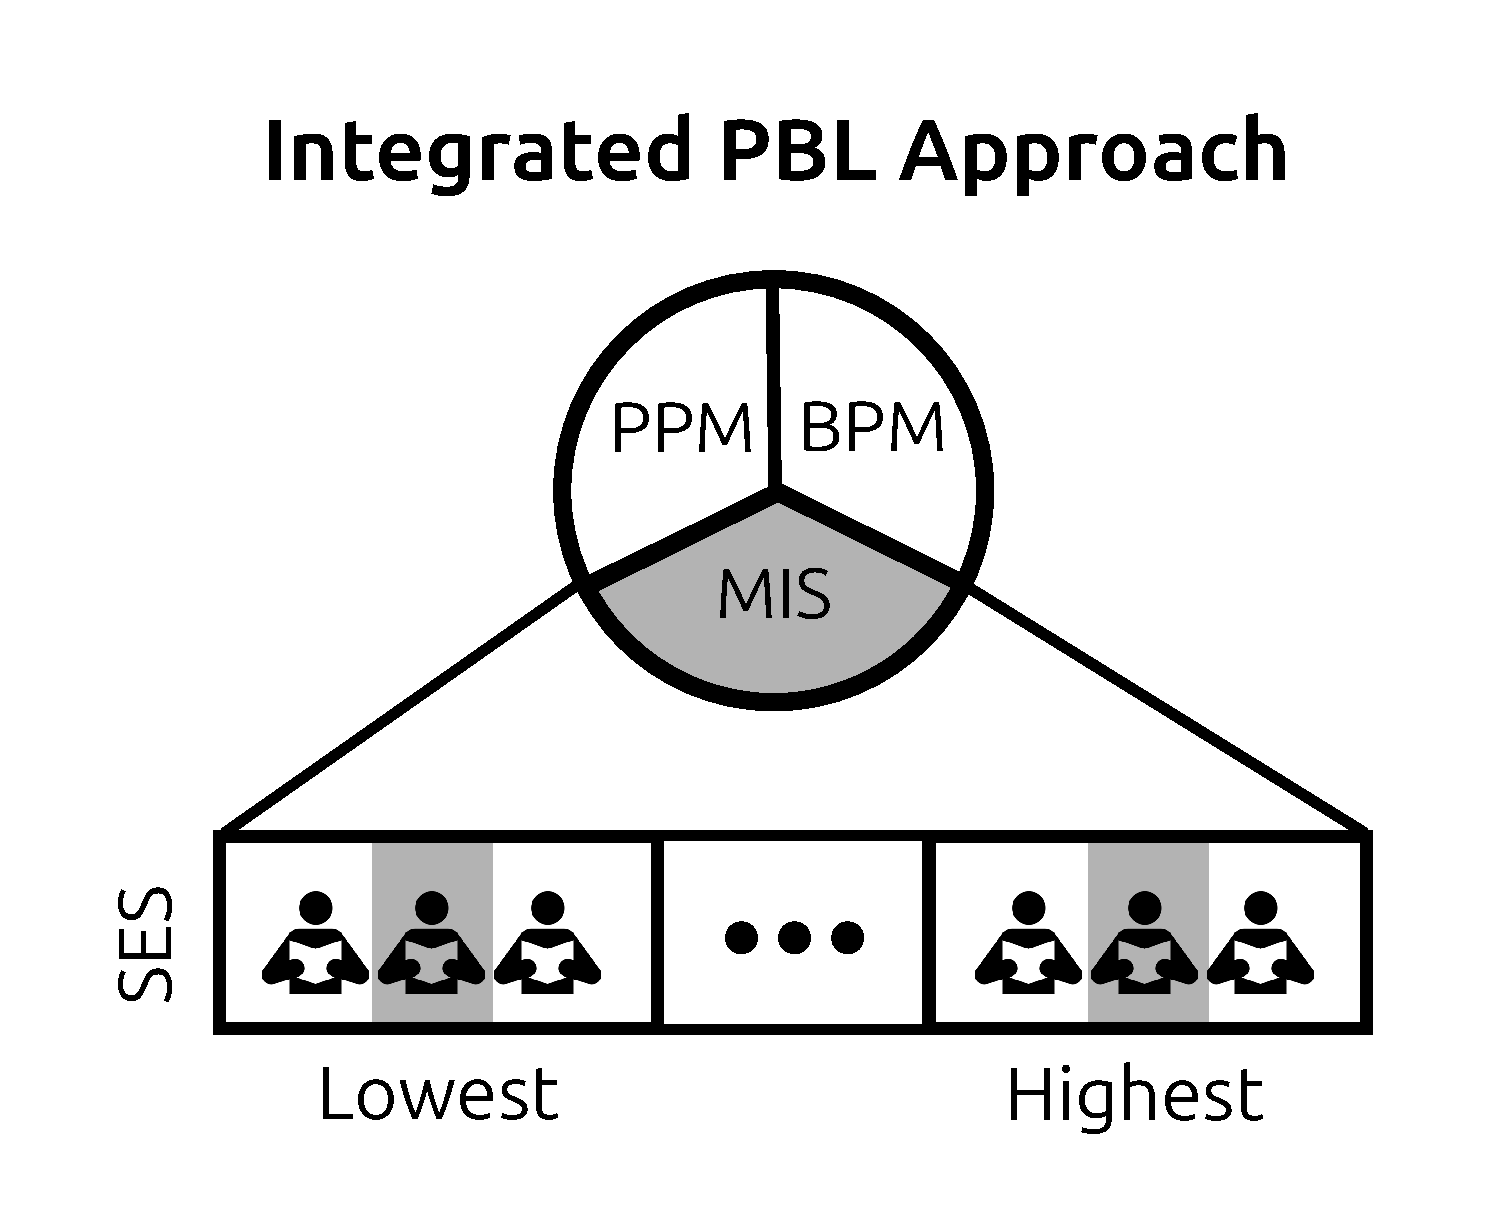
\includegraphics[width=0.9\textwidth]{images/chapter-07/pbl-group.pdf}}

\par\medskip\ABNTEXfontereduzida\selectfont\textbf{Source:} Created by the author (2024).
\end{figure}

This research concentrated more efforts on \gls{MIS} course during the data collection step. My advisor was responsible for facilitating this course in the 2023.1 academic term.

It is essential to highlight that all federal teaching institutions in Brazil adopt affirmative actions for student entry into higher education. As explained in Section \ref{equity-sec:br-context}, these affirmative actions consider various aspects, emphasizing if students attended their whole high school in public teaching institutions. Thus, it should be possible to see significant functioning differences (Section \ref{sen-ss:functioning}) among the students even after four terms of this program.

% \vspace{0.3cm}
% \fbox{
%     \begin{minipage}[htb]{0.9\textwidth}
%         \vspace{0.3cm}
                
%         \colorbox{gray!30}{% create a colored box
%             \makebox[0.975\textwidth][l]{% center the text on the page
%                 \ \ \textbf{Further Writing}
%             }
%         }

%         \vspace{0.1cm}
        
%         \begin{itemize}
%             \item Describing the PBL Framework  \cite{rodrigues:2016}.
%         \end{itemize}

%         \vspace{0.25cm}
        
%     \end{minipage}
% }